% !TEX root = ../main.tex
% !TEX program = xelatex
\section{数据预处理与探索性分析}

\subsection{数据预处理}
本文数据均来自赛题附件。
附件1提供代表日的电价、负载和光伏预测数据；附件2提供2025年全年实际负载和光伏功率；
附件3提供每日多时刻发布的光伏预测；附件4提供全年实际电价。
我们对这些数据进行了\textbf{清洗、格式统一、结构整理和模型所需转换}，确保后续建模与求解的准确性，具体操作如下：

\begin{enumerate}
\item \textbf{数据质量检查。}
首先检查附件1—4中的缺失值、非数值项、异常取值及时间对应关系。
核查后，输入数据不存在需要填补的缺失值。光伏数据中的零值主要对应夜间无发电情况，因此予以保留。对于较大或较小的负载、光伏和电价值，经原始附件核对后也不作删除或修改。

\item \textbf{时间与数据格式统一。}
统一日期和时间格式，并按照“日期—时间”建立负载、光伏和电价之间的对应关系。
针对“0:00+1”等特殊时间标签，按照其真实时间含义进行映射，避免数据错位。对于光伏预报，同时保留预报发布时间和目标时刻，不同发布时间的预报不相互覆盖。

\item \textbf{数据结构整理。}
将原始宽表整理为逐时记录形式，便于不同附件按相同时刻进行匹配。
该过程只改变数据排列方式，不增加、删除或修改原始观测值。对于超出实测时间范围的预报，仅在误差计算时不参与比较，原始预报仍予以保留。

\item \textbf{模型所需转换与核对。}
后续调度以10分钟为一个时段。负载和光伏的功率数据在模型中按
\begin{equation}
E = P \times \frac{1}{6}
\end{equation}
转换为相应时段电量。由于各变量均具有明确的物理意义，本文不进行标准化或归一化处理。最后将整理后的数据与原始附件逐项核对，确保数据数值及对应关系未发生改变。
\end{enumerate}


\subsection{探索性分析}
在完成了数据的预处理与分析之后，我们对数据有以下发现：

\subsubsection*{（1）光伏富余与用电需求存在明显的时间错位}
根据附件1的代表日数据，我们对负载、光伏功率和电价进行日内对比，结果如图\ref{fig:tsxfx_1}所示。

\begin{figure}[H]
    \centering
    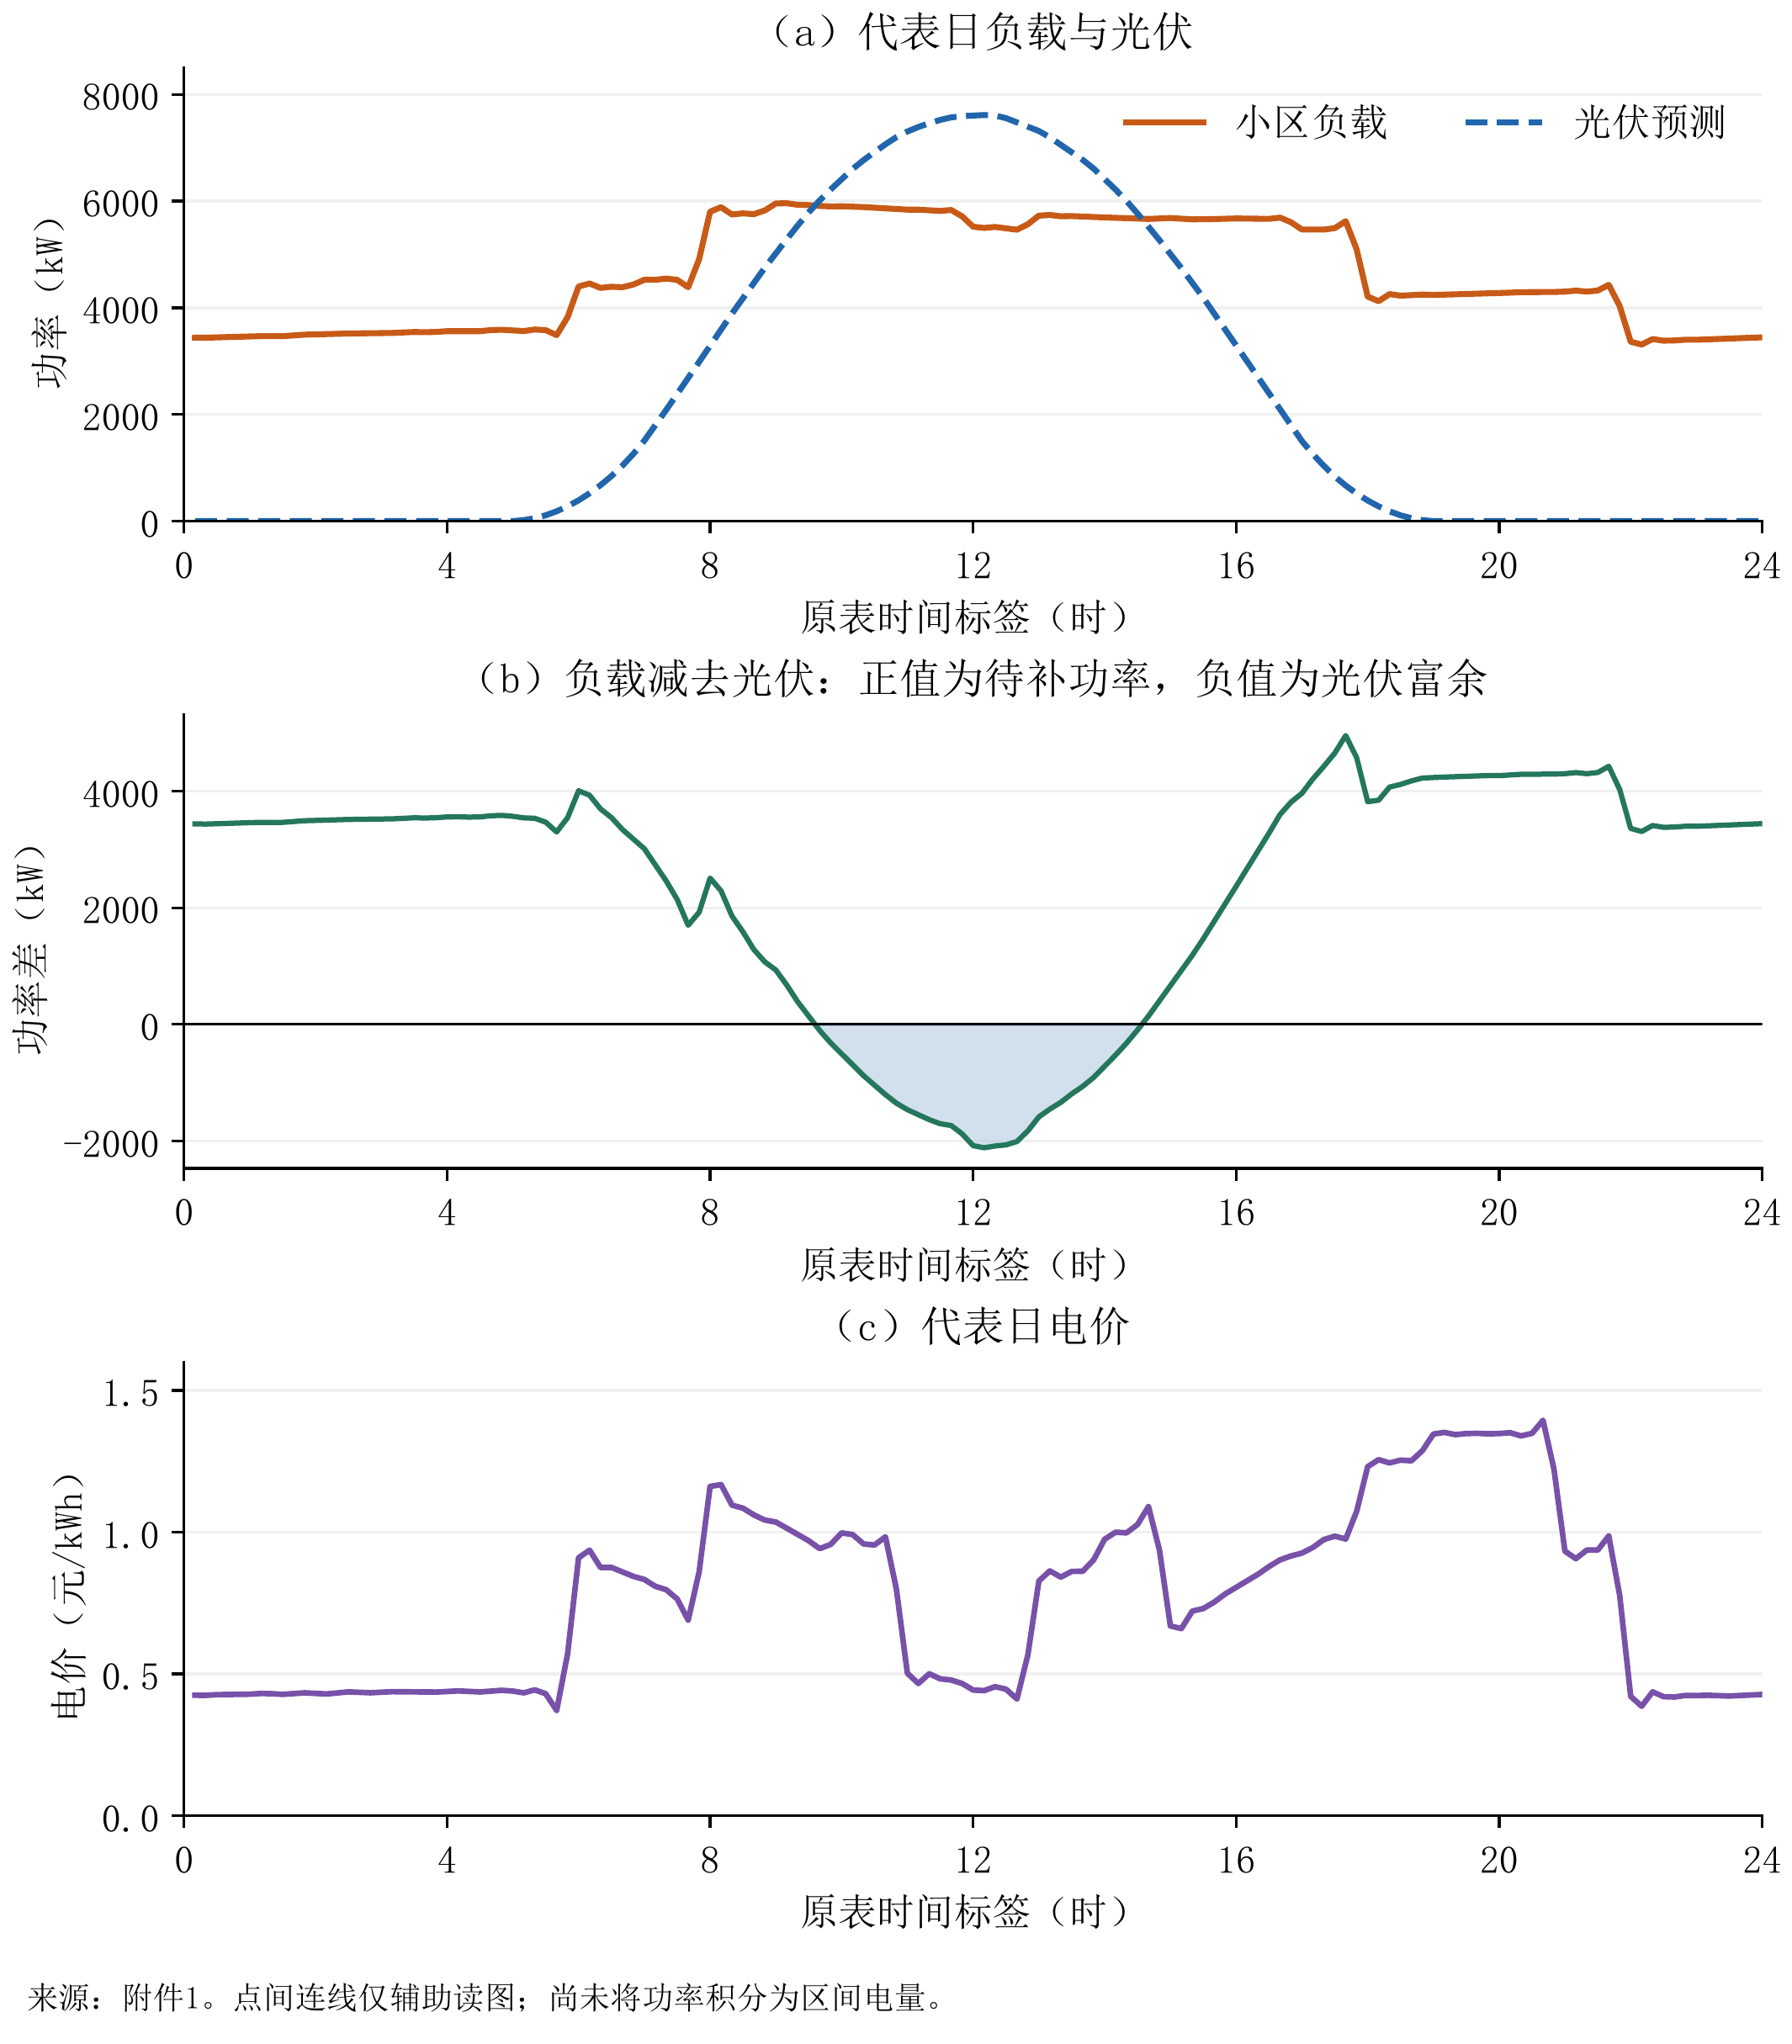
\includegraphics[width=0.8\textwidth]{fig/tsxfx_1.png}
    \caption{代表日供需与电价的时间错配}
    \label{fig:tsxfx_1}
\end{figure}

由图\ref{fig:tsxfx_1}(a)可见，光伏功率主要在白天上升，并在午间达到较高水平，而小区负载全天均保持在较高水平。
进一步由图\ref{fig:tsxfx_1}(b)可见，午间“负载减光伏”为负，说明此时存在光伏富余；进入傍晚后，光伏快速下降，供需缺口重新扩大。
代表日午间最大光伏富余功率约为 \(2100\,\mathrm{kW}\)，而傍晚最大供需缺口接近 \(5000\,\mathrm{kW}\)。

同时，图\ref{fig:tsxfx_1}(c)表明较高电价主要出现在傍晚和晚间，与较大的供需缺口具有一定重合。这意味着高需求时段往往也是购电成本较高的时段。

进一步统计全年数据发现，共有330天出现过光伏功率高于负载的情况，说明午间光伏富余并非个别现象。

因此，\textbf{光伏发电充足的时段与主要用电时段并不一致}。仅比较全天总发电量和总负载无法反映真实运行压力。
储能需要承担跨时段转移电量的作用，将午间富余光伏或低价购电转移到后续高需求、高电价时段使用。


\subsubsection*{（2）负载和光伏均存在年内变化，但变化并不同步}
根据附件2和附件4，我们对全年负载、光伏和电价分别计算每日平均值和月平均值，结果如图\ref{fig:tsxfx_2}所示。

\begin{figure}[H]
    \centering
    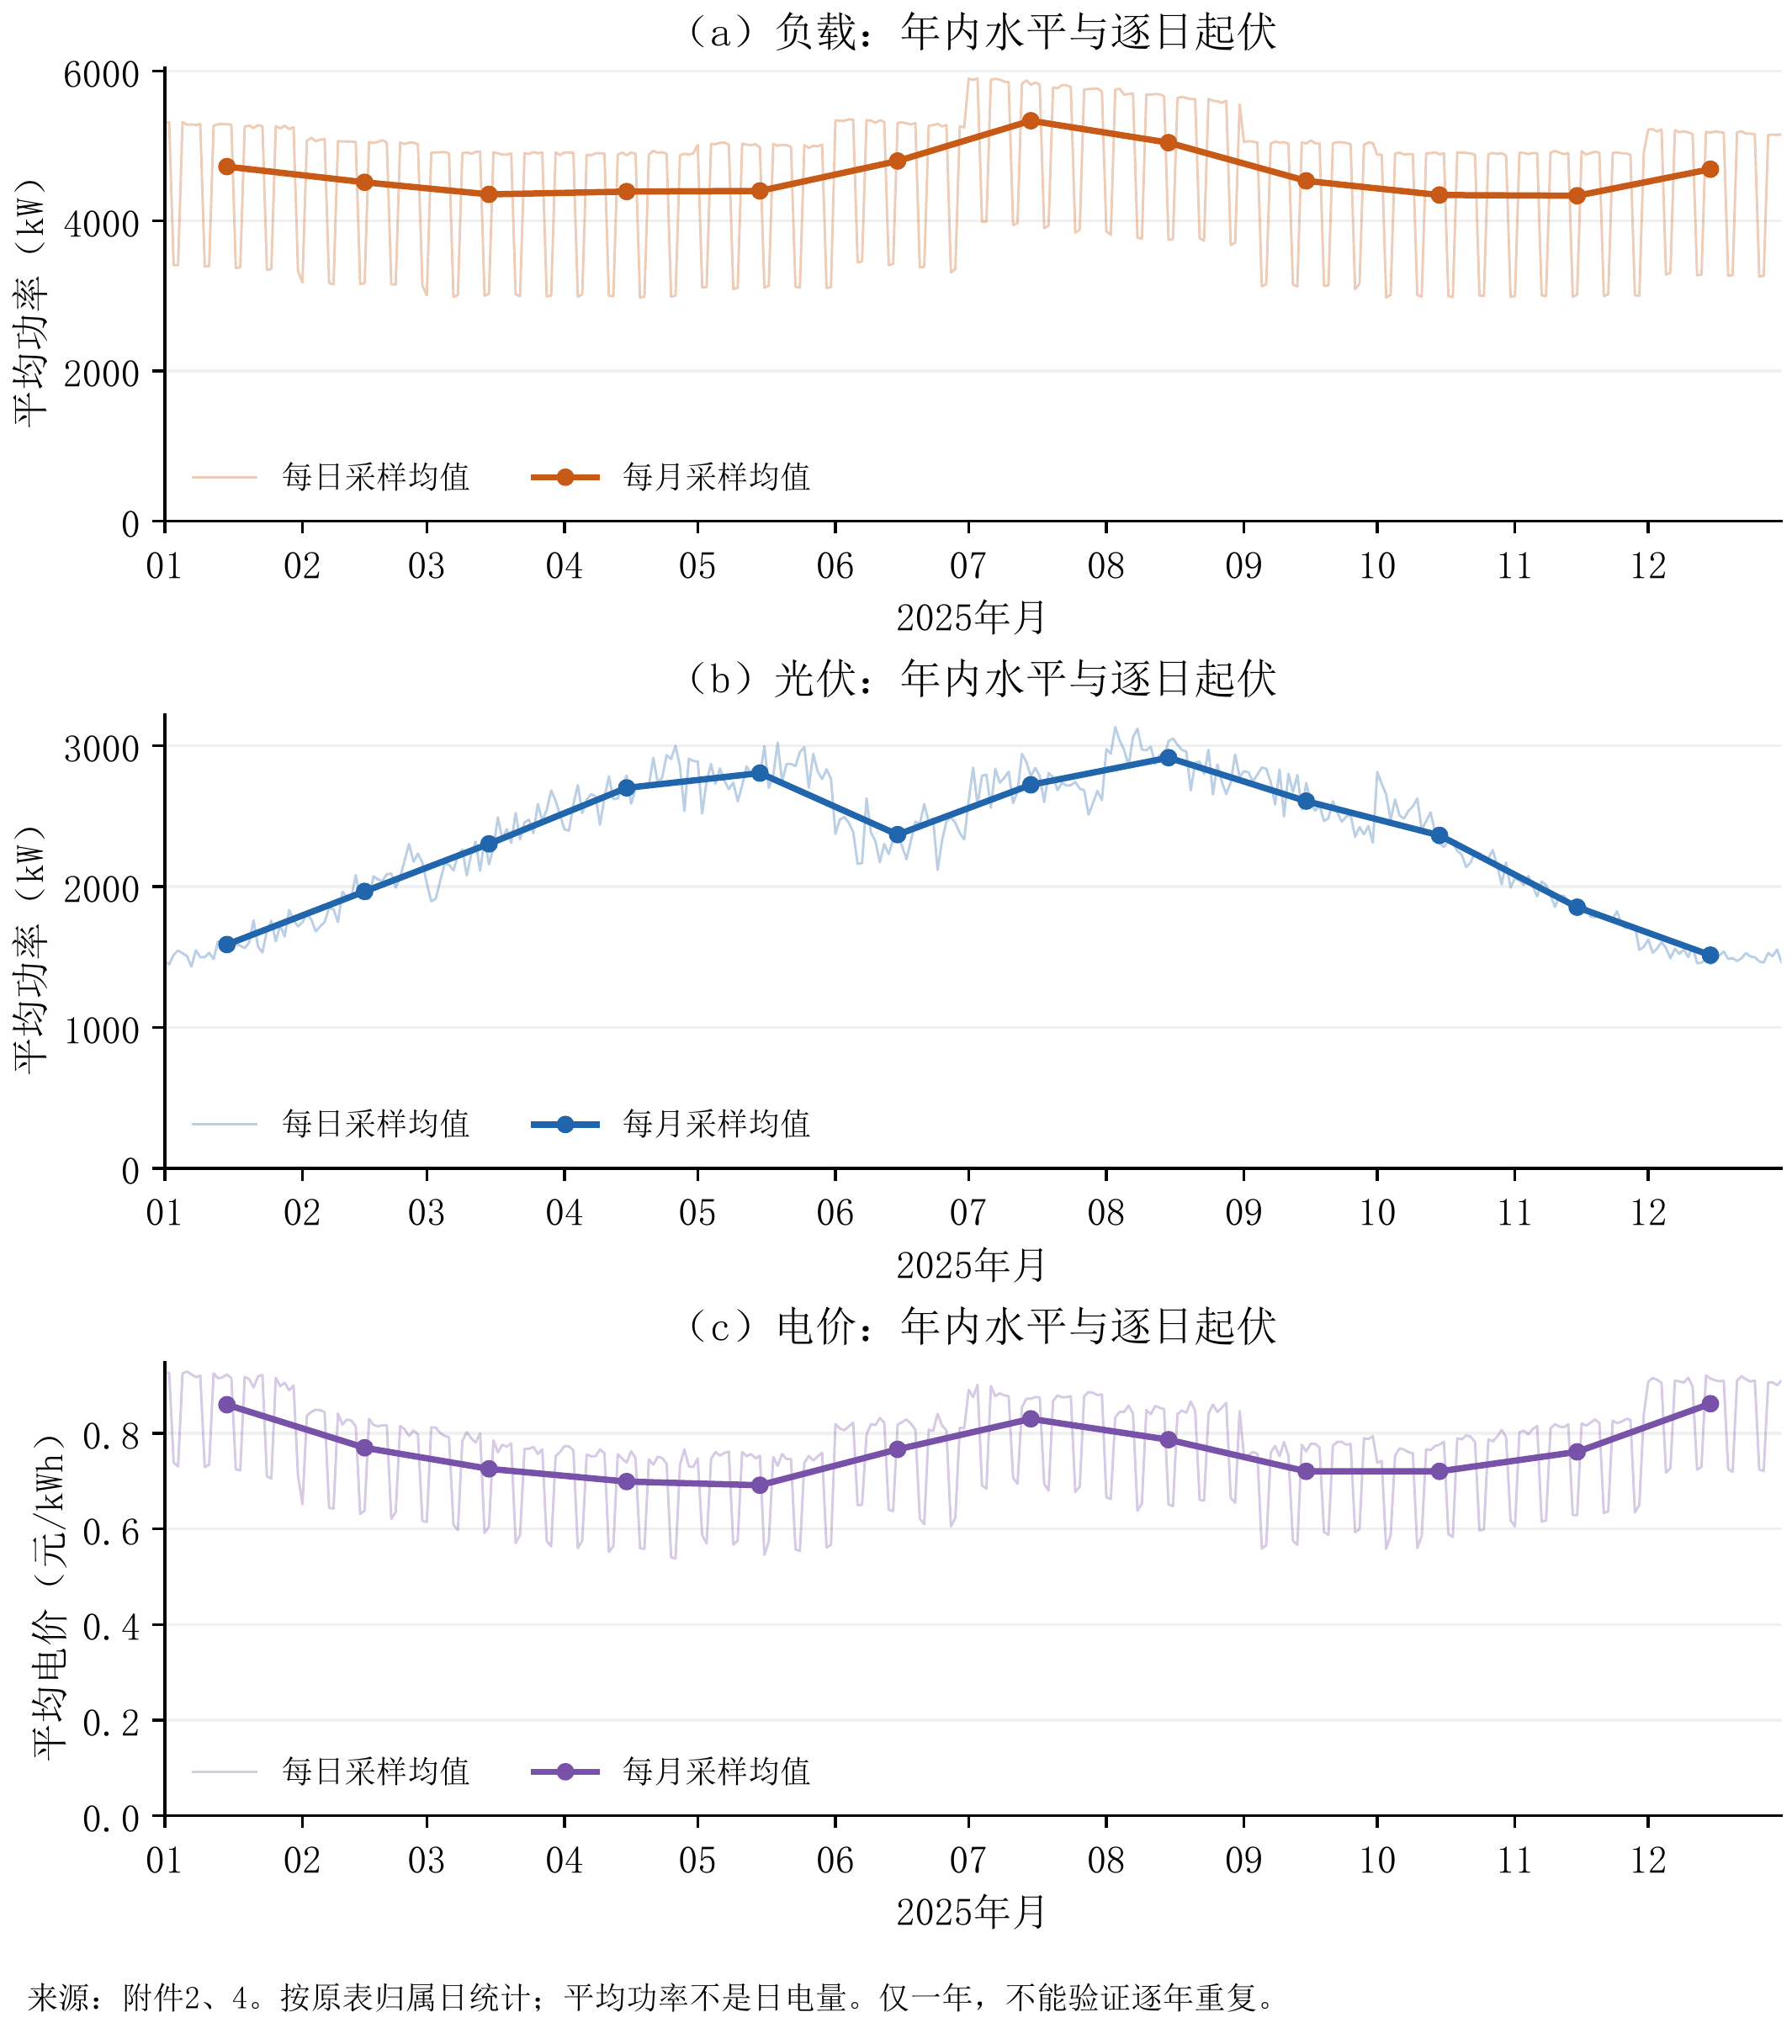
\includegraphics[width=0.8\textwidth]{fig/tsxfx_2.png}
    \caption{代表日供需与电价的时间错配}
    \label{fig:tsxfx_2}
\end{figure}

由图\ref{fig:tsxfx_2}(a)可见，小区负载存在明显的年内变化，夏季整体水平较高；
图\ref{fig:tsxfx_2}(b)显示光伏同样具有季节变化，但其变化趋势与负载并不完全一致。特别是在冬季，负载虽然低于夏季高峰，但光伏出力下降更加明显。

例如，12月平均负载减去光伏后的功率差约为 \(3177\,\mathrm{kW}\)，而5月约为 \(1595\,\mathrm{kW}\)，前者接近后者的两倍。

这说明，\textbf{外网补电压力并不能仅由负载高低决定，还必须同时考虑光伏出力}。
夏季负载虽然较高，但光伏也能提供较多电量；冬季负载并非最高，但由于光伏下降，实际供需缺口仍可能较大。

图\ref{fig:tsxfx_2}(c)还表明全年平均电价同样存在一定的年内起伏。因此，不同月份面临的供需条件和购电环境均有差异，不能将某一天或某一固定购电、充放电策略直接复制到全年。


\subsubsection*{（3）负载具有明显的周重复特征，电价存在跨日波动}
为进一步分析日际规律，我们按实际星期对全年负载和电价进行分组，结果如图\ref{fig:tsxfx_3}所示。

\begin{figure}[H]
    \centering
    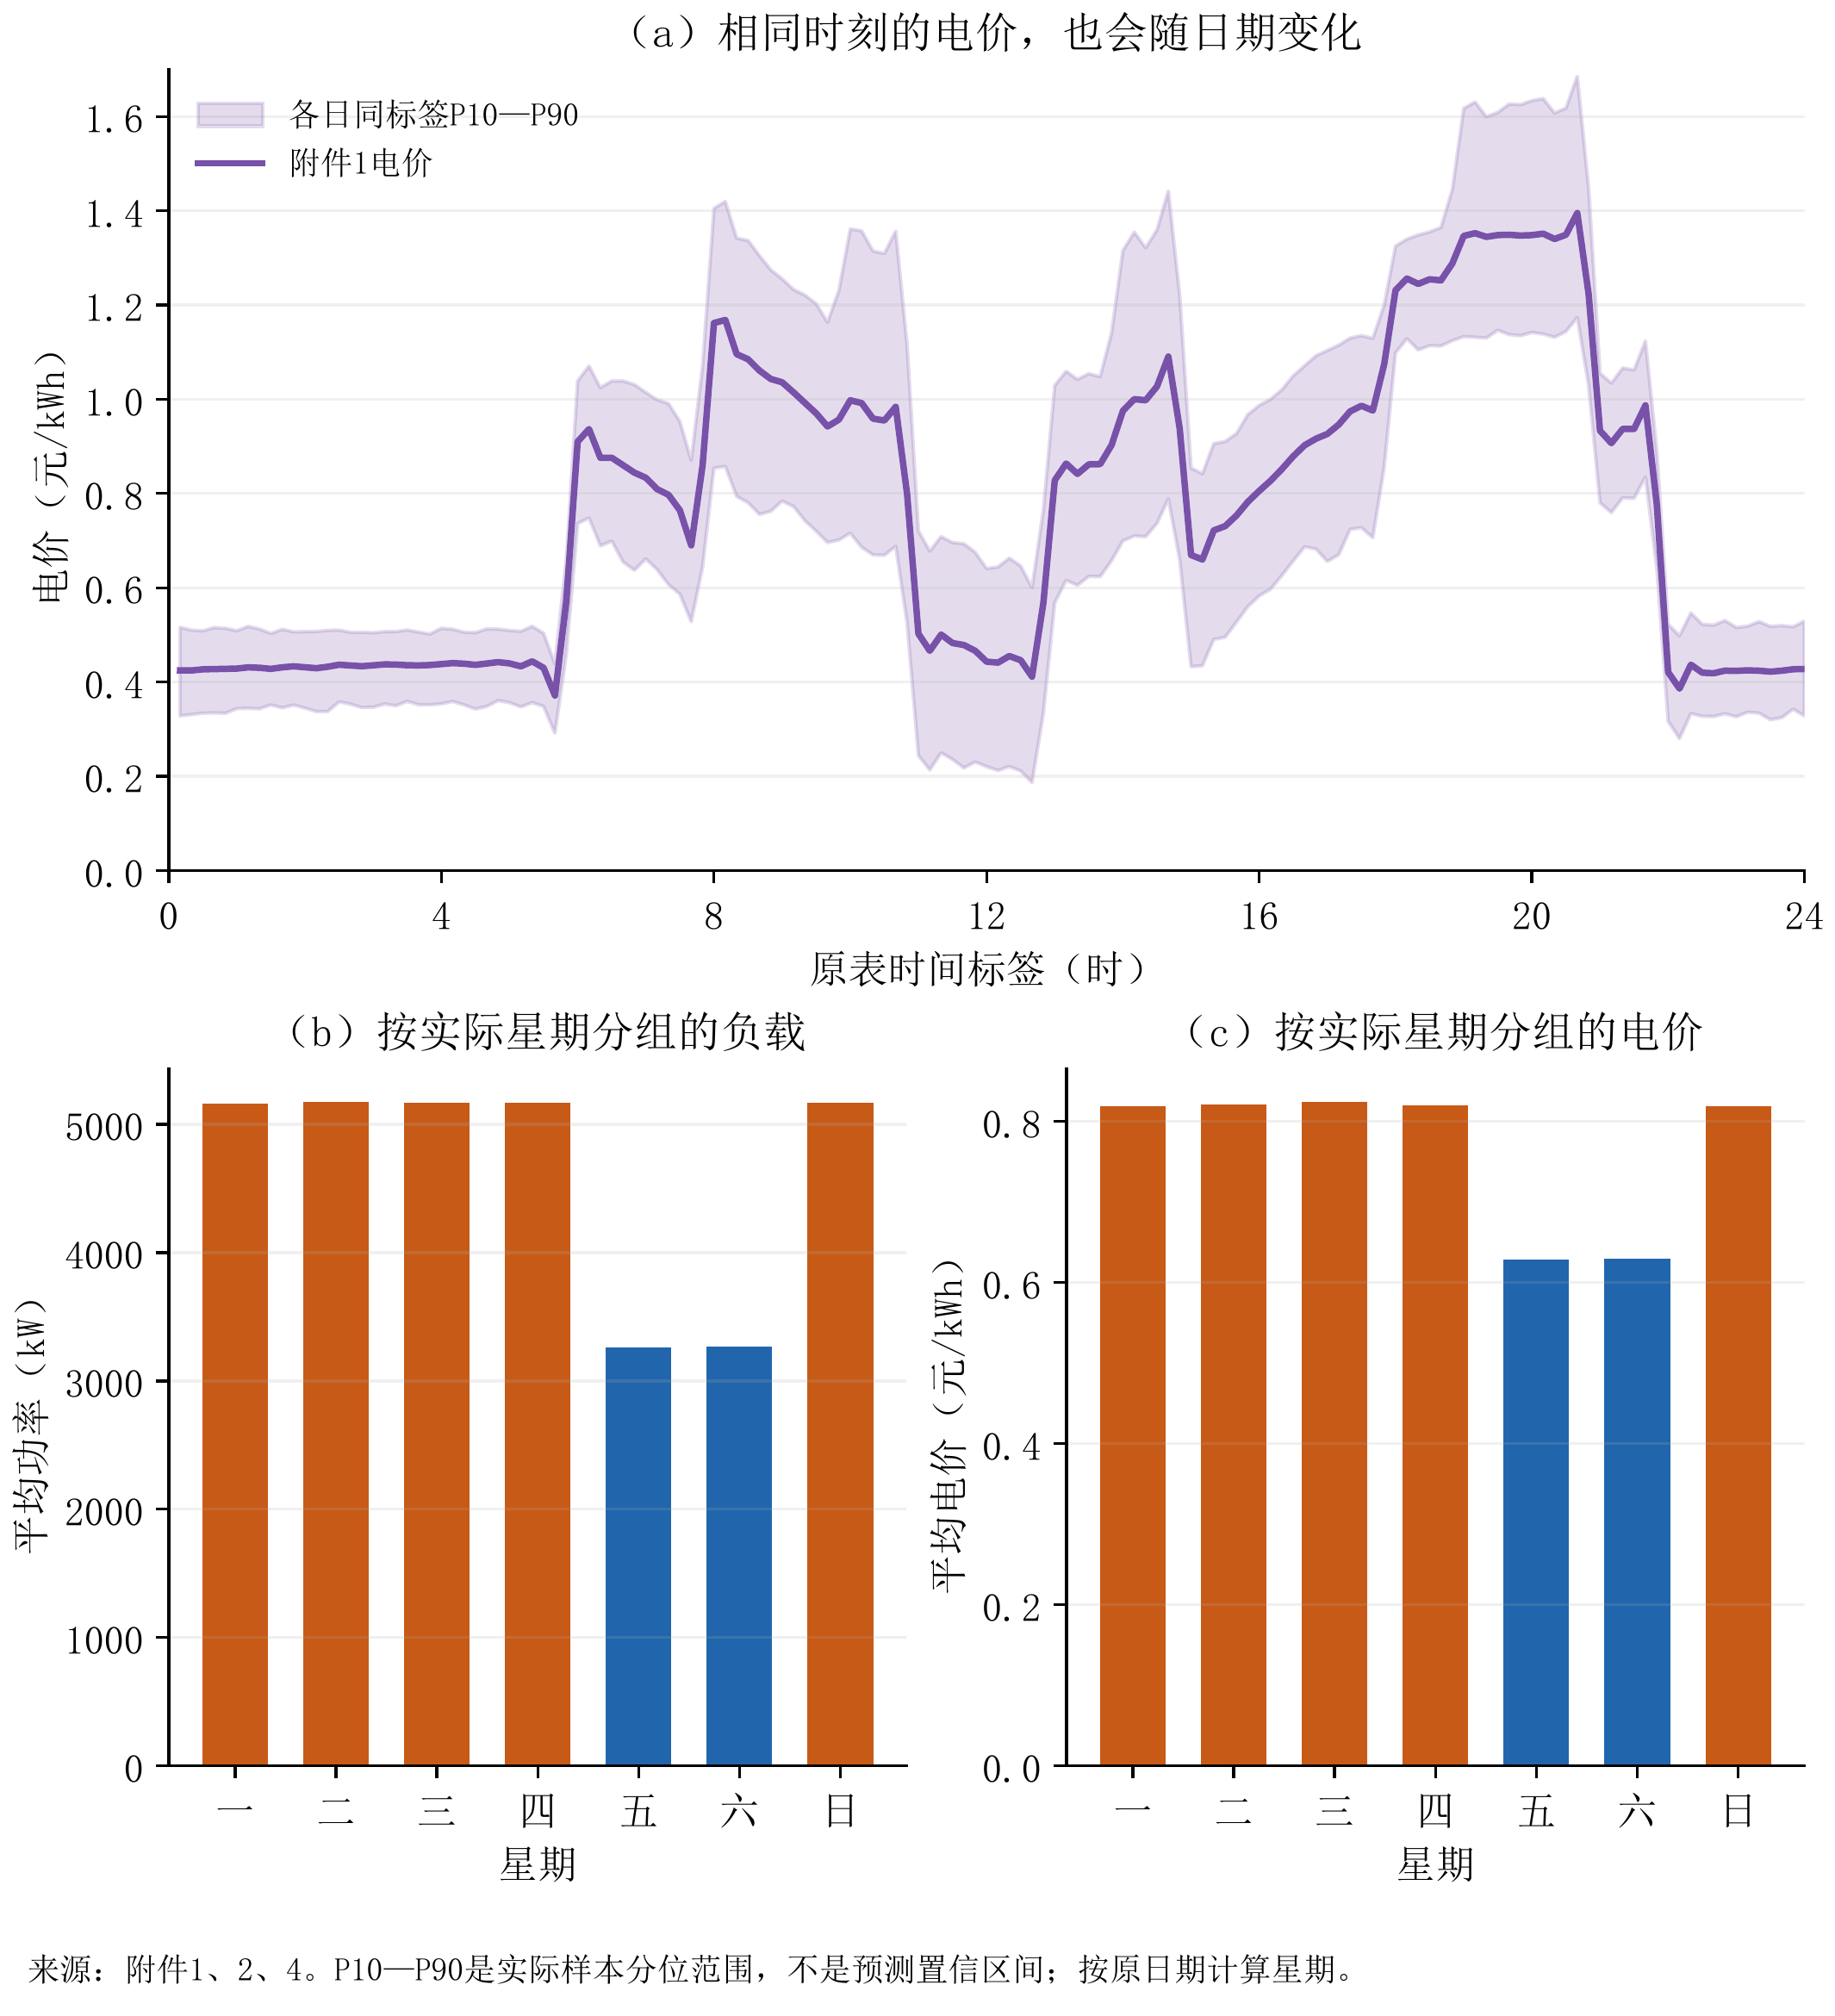
\includegraphics[width=0.8\textwidth]{fig/tsxfx_3.png}
    \caption{代表日供需与电价的时间错配}
    \label{fig:tsxfx_3}
\end{figure}

由图\ref{fig:tsxfx_3}(b)可见，周五和周六的平均负载明显低于其他日期。
统计结果显示，周五和周六的平均负载约为 \(3265\,\mathrm{kW}\)，其余五天约为 \(5168\,\mathrm{kW}\)，前者低约 \(36.8\%\)。
同时，负载与一周前数据的相关性明显高于与前一天数据的相关性，说明负载具有较强的周重复特征。

因此，在利用历史信息判断未来负载时，\textbf{同一星期位置的历史数据具有较强参考价值}，不能只根据前一天的数据进行简单外推。
    
光伏则表现不同。虽然始光伏序列在不同日期之间具有较高相似性，但在扣除各月相同时刻的平均日内轮廓后，其一周相关性接近于零。
这说明光伏曲线的相似主要来自“白天高、夜间低”的共同日内形状，而不是稳定的星期周期。

另一方面，图\ref{fig:tsxfx_3}(a)给出了全年相同时刻电价的第10至第90百分位范围。可以看到，即使处于相同的日内时刻，不同日期的实际电价仍存在明显差异。
图\ref{fig:tsxfx_3}(c)虽然显示不同星期的平均电价存在一定规律，但历史低价时段并不能保证未来同一时刻仍保持相同价格。

因此，\textbf{负载、光伏和电价的历史规律并不完全相同}。负载可以更多参考周重复信息，而光伏和电价仍需考虑较强的日际变化。  


\subsubsection*{（4）日内更新能够提高光伏预报精度，但并非每次更新都更准确}
根据附件3，我们将不同发布时间的光伏预报与相同目标时刻的实际光伏进行匹配，并采用平均绝对误差评价预测偏差，结果如图\ref{fig:tsxfx_4}所示。

\begin{figure}[H]
    \centering
    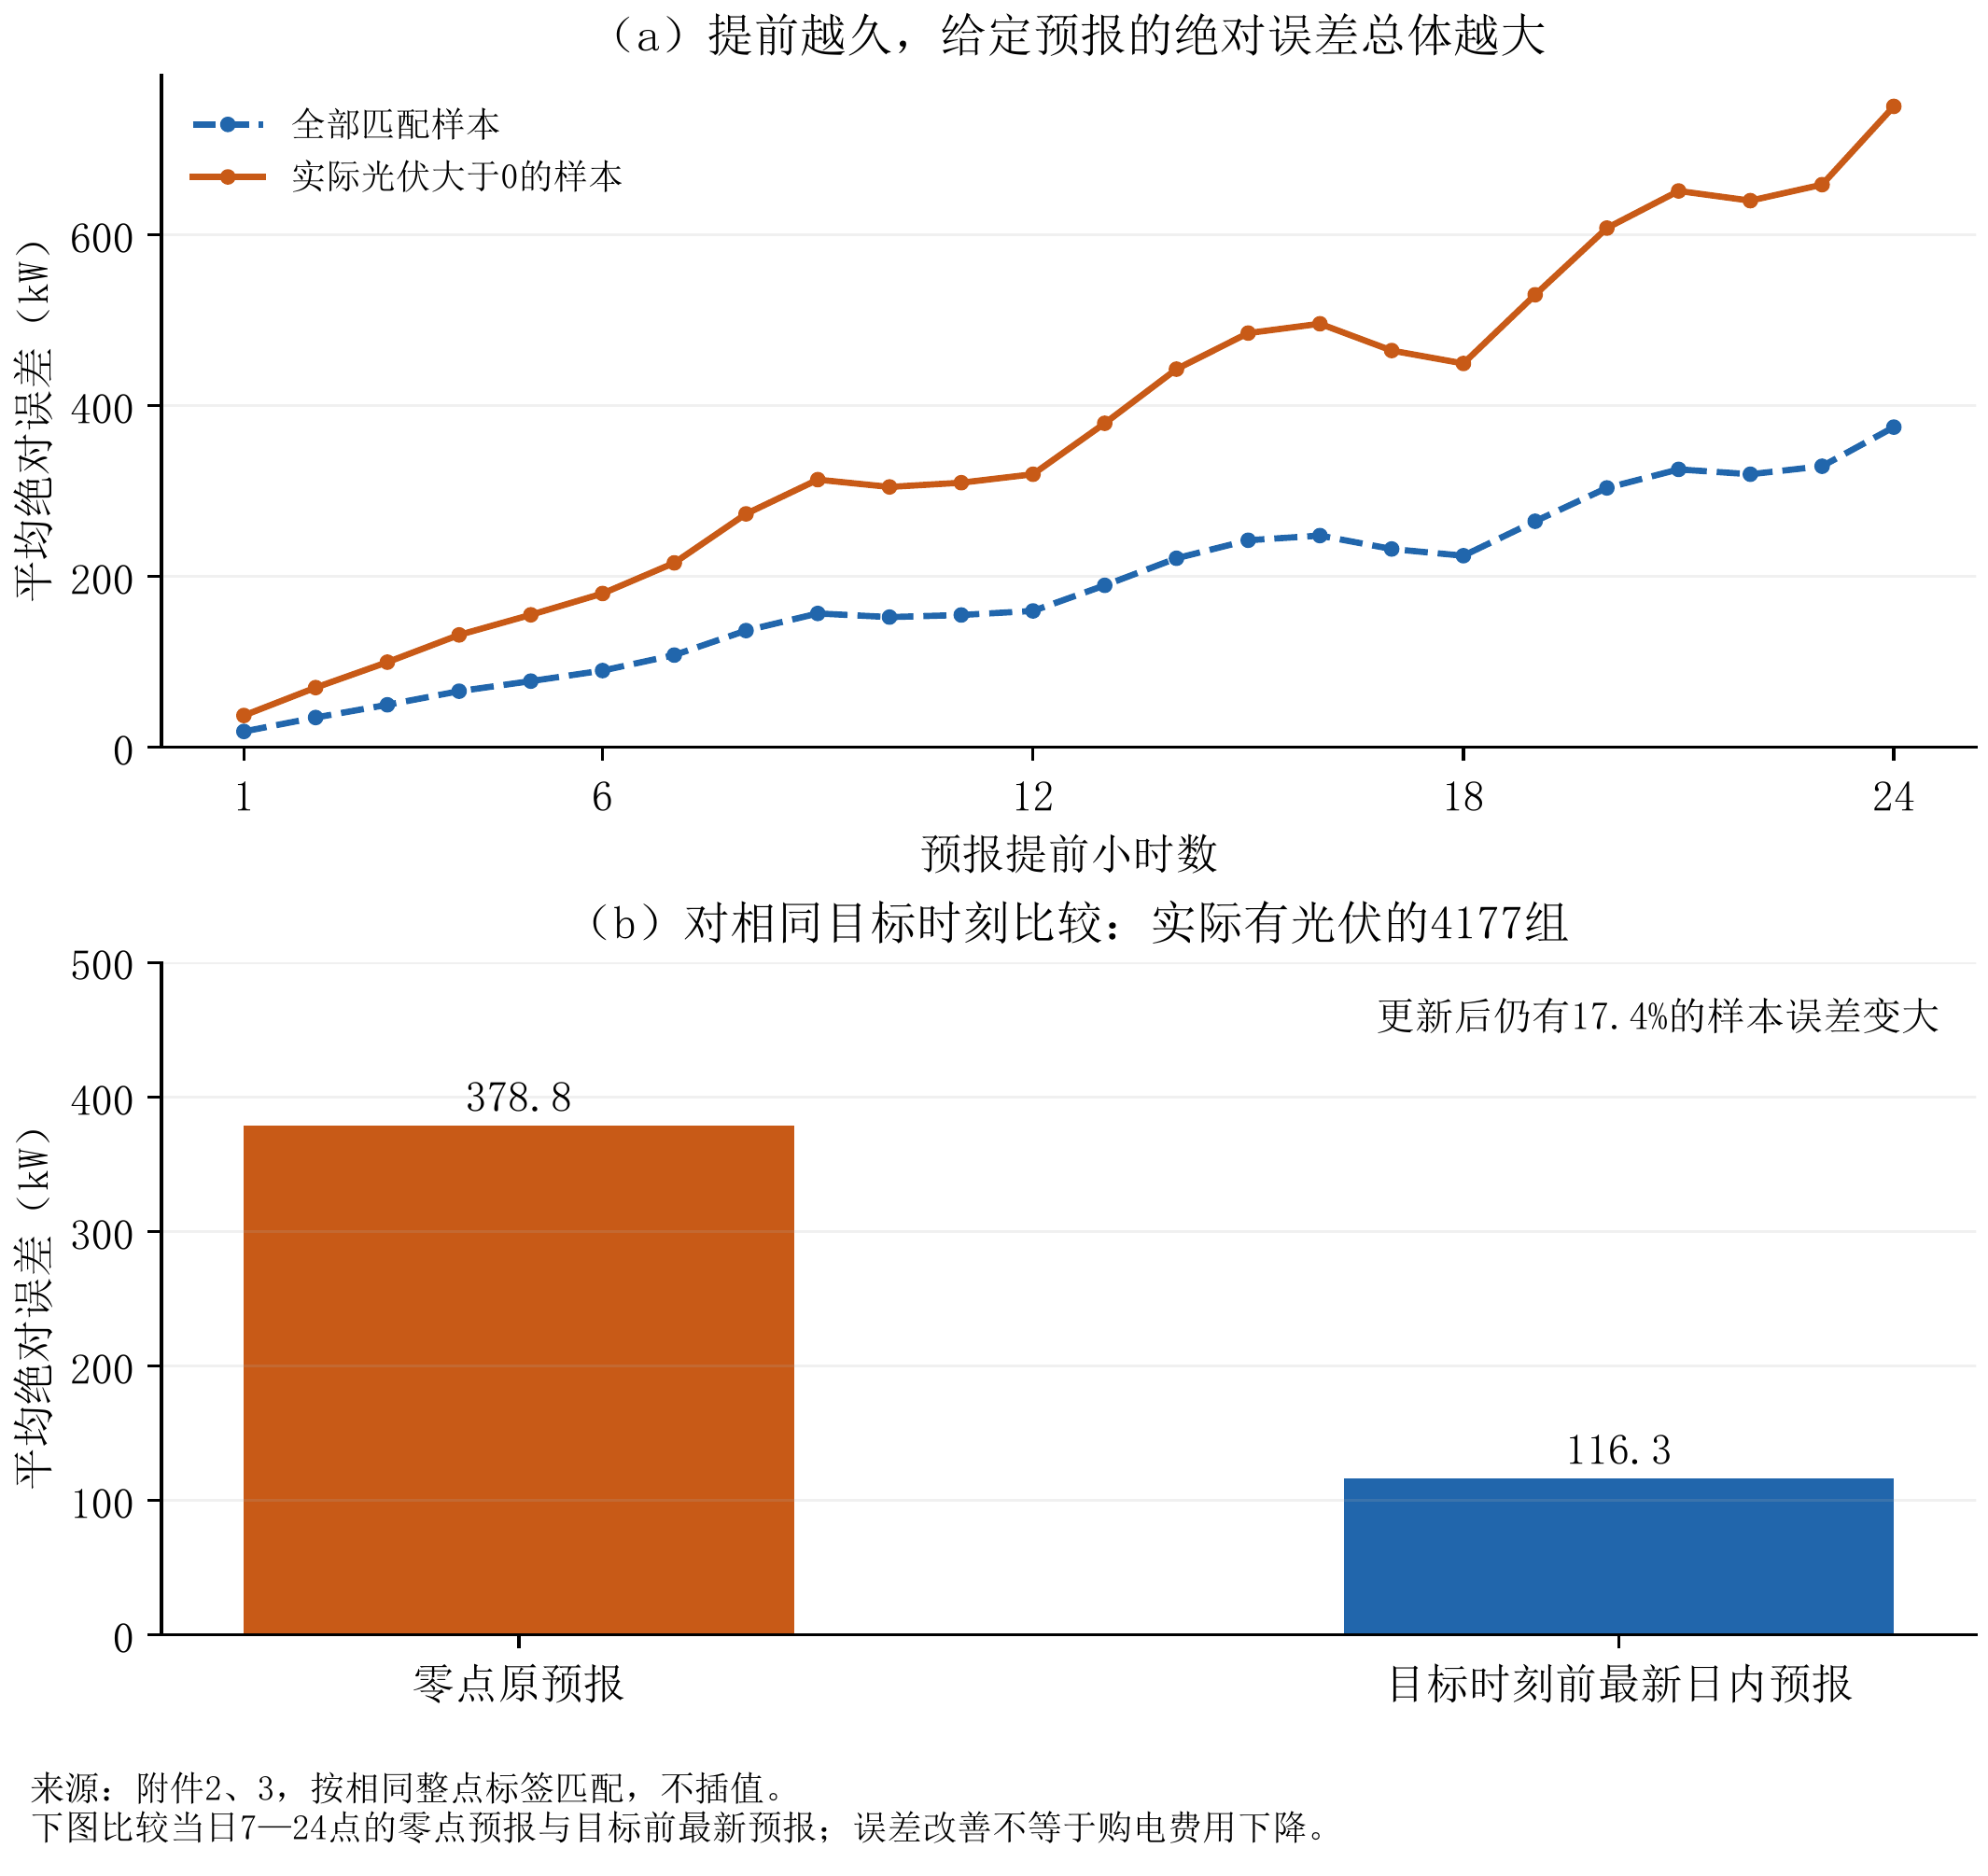
\includegraphics[width=0.8\textwidth]{fig/tsxfx_4.png}
    \caption{代表日供需与电价的时间错配}
    \label{fig:tsxfx_4}
\end{figure}

由图\ref{fig:tsxfx_4}(a)可以看出，随着预报提前时间增加，平均绝对误差总体呈上升趋势，说明距离目标时刻越远，光伏预报通常越不准确。特别是在实际存在光伏出力的样本中，误差更加明显。

为了进一步判断日内更新是否有效，图\ref{fig:tsxfx_4}(b)比较了同一目标时刻下的零点原预报和目标时刻前最新日内预报。
在实际光伏大于0的4177组样本中，平均绝对误差由约 \(378.8\,\mathrm{kW}\) 降低至 \(116.3\,\mathrm{kW}\)，下降约 \(69\%\)。这说明日内更新总体上明显提高了预报精度。

但图\ref{fig:tsxfx_4}(b)同时显示，仍有约 \(17.4\%\) 的样本在更新后误差反而增大。因此，新的预报虽然总体更准确，但\textbf{并不意味着每次更新都一定优于原预报}。

此外，预测误差降低也不等于购电费用按相同比例降低。如果新的预测偏差可以由储能设备自行吸收，则调整购电计划未必划算；
只有当更新后的预测明显改变未来供需缺口，并且节省的紧急购电费用能够覆盖调整成本时，日内预报更新才具有实际经济价值。